\documentclass[twocolumn]{article}
\usepackage{graphicx}
\usepackage{wrapfig}
\newcommand{\degree}{\ensuremath{^\circ}}
%\linespread{1.6}
\title{Artist Classification with Stylometry and Support Vector Machines}
\author{Ari Brown, Drew Gleeman, and Mike Micatka}
\date{\today}
\begin{document}
  \maketitle

  \section{Introduction}
  \subsection{Problem}
  The problem with being STEM students is that we have an incredibly poor ability
  to recognize artists from paintings. However, as with most problems in the
  modern age, they are easily solved with computers and math. Our specific problem
  is: given a painting and two possible artists, which artist made the painting?
  The problem itself is interesting although not important. It approaches the
  field of forgery detection, as our project is forgery detection at its most
  basic level: artist classification. \\
  
  We are going about this project by using a machine learning algorithm (Support
  Vector Machine, SVM) to make an educated estimate on who the artist is. With
  zero training, the computer would make simply a random guess. To turn this guess
  into an educated estimate, we train it on data from six different features of
  each painting, telling the computer to which artist the features belong to.
  SVM can only make a decision based on one feature, so we run the SVM once for
  each feature and then we combine the outcomes of each feature using a weighted
  voting algorithm, where each feature's result gets a certain number of votes,
  and the winner is then declared by the program with a ``sureness'' factor.

  \subsection{Previous Work}
  There was a similar project done by undergraduate students at Stanford
  University in a machine learning class that focused on the machine learning
  aspect. Blessing and Wen used twelve different features to classify their
  data, with overlap on five of them with ours. Coincidentally, they chose to
  use the same machine learning algorithms as we did, which were a Bayesian
  Analyzer and Support Vector Machines. \\
  
  Our implementation differs from the reference implementation because we use
  fewer features to base our artist-selection decisions on, and we have
  different weights for our final decider. Trivially, we also used different
  data, overlapping with only two of the artists. \\

  Our implementation is better than the reference implementation because we
  make use of a weighted council-like approach to produce a single answer
  based on all of our styolmetrics. We also use cross validation to get better
  training and more generalized results. Cross validation allows us to reuse
  data to achieve better results by doing more training.

  \section{Technical Solution}
  \subsection{Summary}
  In its simplest form, our program takes two artists, trains the machine on
  40\% of the data, and then uses the remaining 60\% to test the results while
  recording the accuracy for estimating each artist. This gives us a measure on
  both false positives and false negatives, both of which are important.

  \subsection{Data}
  We chose four artists (Rembrandt, Pollock, Monet, and Picasso) and selected
  roughly 100 works from each artist. We chose each artist for their fame and
  peculiarities. Picasso was an interesting artist to choose, simply because his
  style has ranged from realism as a youth to cubism later in his life.
  Rembrandt is an artist we had seen mentioned in many papers, so we figured
  that it would be important to include him in our work. Pollock was chosen as
  he was an abstract painter with creative uses of colors that focused around a
  certain theme. Monet was selected as he was an impressionist painter who did
  many plein-air landscapes.

  \subsection{Weighted Combination}
  On a more technical level, the program also takes information on the weights
  of each feature and the threshold for ``sureness'', in which if the resulting
  sureness fails to meet the sureness, the program will produce a symbol which
  equates to not knowing. As each individiual styolmetric feature gives its
  opinion on which artist produced the painting, the program weights the result
  as -1 or 1, depending on the determined artist. When all the stylometries have
  produced a result, the values are then weighted respectively according to the
  inputted weight matrix. The weighted values are then summed, and the final
  output is compared with the ``sureness'' threshold, and a final decision on
  the artist is produced. This process is completed for each painting. To speed
  this process, the stylometric data, an invariant, is produced ahead of time
  and stored in a handwritten file-system database. \\

  \subsection{Cross Validation}

  \subsection{Histogram of Oriented Gradients}
  The histogram of oriented gradients stylometric, or HoG, is based on the
  direction of intensity changes in cells across an image. The idea behind it is
  that changes in intensity mark feature changes, and so a histogram for a small
  cell is produced based on each pixel. The histograms of each cell are then
  compiled into one, which is the final stylometric result. Which used a
  handwritten implementation that was heavily influenced from a different
  source.

  \subsection{Edge Detection}

  \subsection{Local Binary Patterns}
  Local Binary Patterns are patterns that appear in numbers when checking the
  intensity of individual pixels. It is commonly used in texture identification,
  so the logic behind using it is that it would identify pixelated artwork such
  as that which Seurat is famous for (although Seurat's paintings were not used
  in this project). We used a handwritten implementation.

  \subsection{Corner Detection}
  Corner detection simply detects corner in the image. We used a handwritten
  implementation the detects the corners for a given threshold. The logic behind
  using this stylometric is that we will be able to tell if an artist prefers to
  use sharp contrast in two directions in their work. It is an extension of Edge
  Detection, in that regard. \\

  \subsection{Color Histogram}
  We did not expect much from this stylometric, but wanted to include it because
  it could shed light on an artist's overall color intensity. It was calculated
  by averaging the red, green, and blue values, respectively, for all pixels.
  The overall intensity of each pixel was also calculated. The motivation behind
  this was to observe an artist's overall intensity, as aforementioned, but also
  to discern any color preferences, however slight. \\

  \subsection{SIFT}
  SIFT or scale-invarient feature transform is an algorithm that is used to
  describe and locate features in images. The first part of this algorithm
  involves finding the keypoints which is done by finding the maxima/minima of
  the Difference of Gaussians (DoG) at different scales. Features can be examined
  at different scales by changing the size of the $\sigma$ when finding the DoG.
  By examining features at different scale levels features that would otherwise
  be overlooked can be found. This is useful for art identification because
  the different styles of artists can be subjectively determined by the patterns
  that exists at multiple levels, from brushstrokes to the overall theme of a
  painting. \\
  
  The SIFT algorithm that was utilized was from the VLFeat library but a custom
  Bag of Words model in order to generate sets of histograms that could then be
  used for our machine learning algorithm. SIFT finds different features and
  represents them as a 128-dimensional vector. We combined all of the SIFT features
  from our training set and clustered them into 10 different groups using k-means
  clustering. We then generated histograms of frequency for all of the images, both
  training and testing alike, of each of the feature clusters found in the training
  images of both artists. We can then use the histograms of the training set to
  train the SVM and the histograms of the testing images to classify using the
  trained SVM.

  \subsection{Blob Detection}
  Blob detection is a technique in which we calculate the centers of points of
  interest that have large intensity changes. The radius of a blob measures
  how far that intensity goes before changing drastically. This means it would
  be a great stylometric for measuring the presence of overall features that
  would mark a painting as visually distracting, such as still lives and Van
  Gogh's famous sunflower painting. \\

  We were, regrettably, unable to include blob detection in our project
  because we could not produce a fast enough implementation to run on over 400
  images. Our issue lies in the non-maximum suppresion algorithm we have.

  \subsection{Fourier Spectral Analysis}
  Fourier Spectral Analysis is a common technique that was suggested to us by
  Dr. Dan Rockmore as a replacement for blob detection. Fourier spectral
  analysis returns Fourier coefficients for the image, where low frequency
  values represent background and high frequency values represent foreground
  and texture. The resulting matrix is in the shape of the original image
  (with the pixels having a change of basis performed on them, so the values
  do not match up at all), which means it is impossible to train the SVM
  algorithm on the raw FSA data. As an attempt to solve this, we tried taking
  the covariance of the data, which also unfortunately returned a matrix that
  was ultimately based on the size of the original image. \\

  We decided not to include Fourier spectral analysis in our final form
  because we could not figure out a way to faithfully represent the Fourier
  coefficients, and the overall results were not good enough to be included;
  they were little more than random guesses.

  \section{Experiments}
  This one shows stuff.
  \begin{figure}
    \begin{center}
      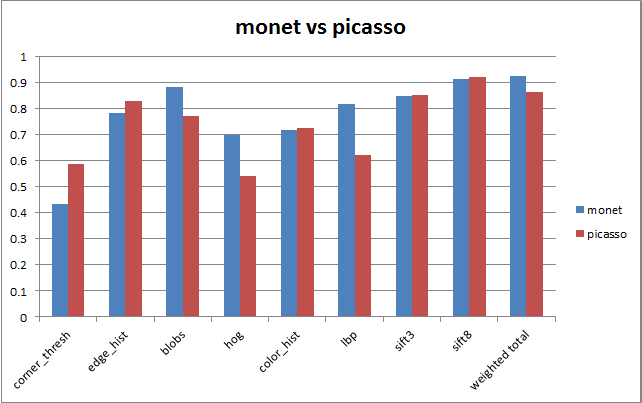
\includegraphics{graphs/monet_picasso.png}
    \end{center}
  \end{figure}

  This one shows stuff.
  \begin{figure}
    \begin{center}
      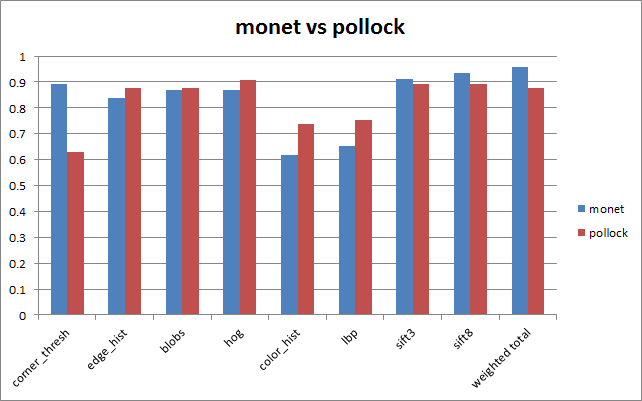
\includegraphics{graphs/monet_pollock.png}
    \end{center}
  \end{figure}

  This one shows stuff.
  \begin{figure}
    \begin{center}
      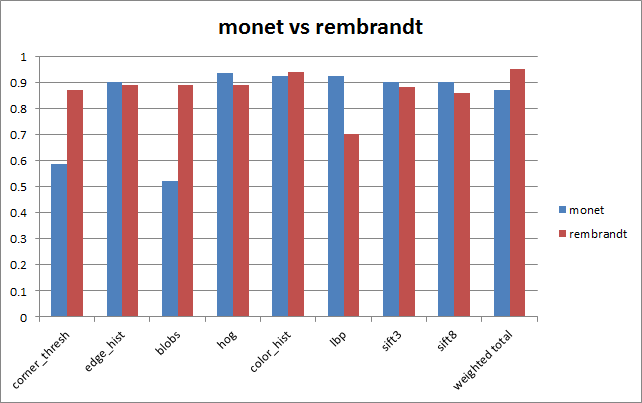
\includegraphics{graphs/monet_rembrandt.png}
    \end{center}
  \end{figure}

  This one shows stuff.
  \begin{figure}
    \begin{center}
      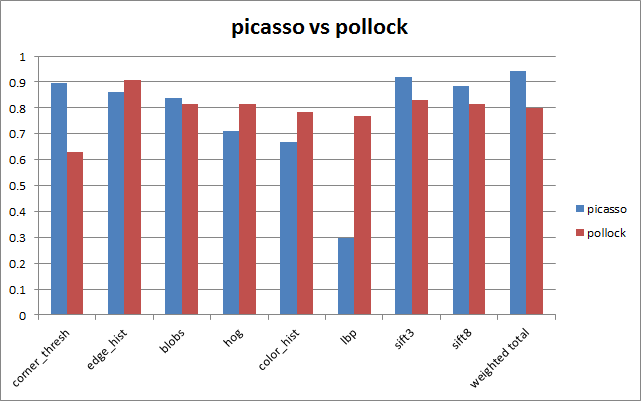
\includegraphics{graphs/picasso_pollock.png}
    \end{center}
  \end{figure}

  This one shows stuff.
  \begin{figure}
    \begin{center}
      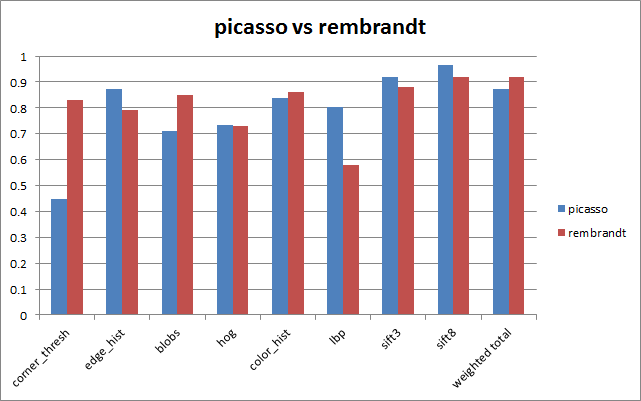
\includegraphics{graphs/picasso_rembrandt.png}
    \end{center}
  \end{figure}

  This one shows stuff.
  \begin{figure}
    \begin{center}
      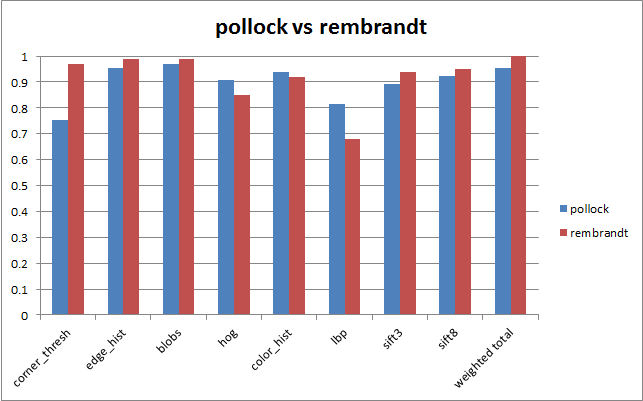
\includegraphics{graphs/pollock_rembrandt.png}
    \end{center}
  \end{figure}

  \section{Conclusions}

  \begin{thebibliography}{1}
    \bibitem{blessing} Blessing, A. and Wen, K.,
    2010,
    \emph{Using Machine Learning for Identification of Art Paintings}.
  
    \bibitem{empirical} Hughes, J. M., Mao, D., Rockmore, D. M.,
    Wang, Y., Wu, Qiang.,
    NOVEMBER 2012,
    \emph{Empirical Mode Decomposition Analysis for Visual Stylometry}.
    IEEE TRANSACTIONS ON PATTERN ANALYSIS AND MACHINE INTELLIGENCE,
    VOL. 34,
    NO. 11.
  
    \bibitem{drawing} Hughes, J. M., Graham, D. J., Rockmore, D. M.,
    \emph{Stylometrics of artwork: uses and limitations}.
  
  \end{thebibliography}

\end{document}

